\documentclass[iop,apj]{emulateapj}
\pdfoutput=1 %for arxiv submission to use pdf
\usepackage{apjfonts}
\usepackage{natbib}
\usepackage{epstopdf}
\usepackage{amsmath,amstext,textcomp}
\usepackage[breaklinks,colorlinks,citecolor=blue,linkcolor=magenta]{hyperref} 
\usepackage[all]{hypcap} %Links go to figures. This breaks deluxetables; use \capstartfalse \capstarttrue around deluxetables to fix it.
\renewcommand{\sectionautorefname}{\S} %for \autoref
\renewcommand{\subsectionautorefname}{\S} %for \autoref
\renewcommand{\subsubsectionautorefname}{\S} %for \autoref

\newcommand{\Reff}{R$_{\rm eff}$}
\newcommand{\Msun}{M$_{\odot}$}

%\renewcommand{\deg}{\ensuremath{^{\circ}}\xspace} %defines a degree symbol

\shorttitle{CCGs in the RESOLVE Survey}
\shortauthors{Snyder et al.}

\begin{document}

\title{The Formation and Evolution of Compact Core Galaxies in the RESOLVE Survey}
\author{Elaine M. Snyder\altaffilmark{1}}
\author{Sheila J. Kannappan\altaffilmark{1}}
\author{Dara J. Norman\altaffilmark{2}}
\author{Mark N. Norris\altaffilmark{3}}
\author{Callie Hood\altaffilmark{1}}
\author{Ashley S. Bittner\altaffilmark{1}}
\author{Christine Ray\altaffilmark{1,4}}
\author{Kathleen D. Eckert\altaffilmark{1}}
\author{the RESOLVE Team}
\affil{$^1$University of North Carolina at Chapel Hill}
\affil{$^2$National Optical Astronomical Observatory}
\affil{$^3$University of Central Lancashire}
\affil{$^4$Rutgers, The State University of New Jersey}
\begin{abstract}
We analyze the complete set of compact core galaxies (CCGs) in the volume-limited RESOLVE survey to investigate the formation and evolution of compact galaxies across a broad statistical distribution of environments. CCGs include both compact ellipticals (cEs) and compact cores surrounded by an envelope of gas and stars, which may represent earlier or later evolutionary stages of cEs. We select CCGs to have core-only radius $<800$pc, an upper limit that encompasses all of the similarly compact stellar systems (ultra compact dwarfs, cEs, nucleated dwarf ellipticals) included in the Archive of Intermediate Mass Stellar Systems (AIMSS) catalog. CCGs naturally occur in a range of environments from isolated to cluster. With GALEX NUV data, we derive star formation histories and find that a significant number of CCGs have recently formed stars. We compare velocity dispersions of CCGs derived from Gemini IFU data to velocity dispersions of other RESOLVE galaxies derived from SOAR spectroscopy. We search for CCGs offset to higher or lower dispersion in the dispersion-stellar mass relation, which may indicate tidal stripping or dissipative formation, respectively. Initial results show several CCGs following the dissipative formation track.
\end{abstract}

\keywords{galaxies: formation; galaxies: evolution}
\maketitle

%%%%%%%%%%%%%%%%%%%%%%%%%%%%%%%
%%%%%%%%%%%%%%%%%%%%%%%%%%%%%%%
\section{Introduction}
\label{intro}

\noindent The term compact stellar system (CSS) composes a class of galaxies that spans the radius range ($\sim10 - 800$ pc), lying between globular clusters (GCs) and normal elliptical galaxies (Es). Different types of CSSs include ultra compact dwarf galaxies (UCDs; \citet{Phillipps2001}), compact elliptical galaxies (cEs; \citet{Faber1973}), dwarf elliptical galaxies (dEs), and nucleated dwarf elliptical galaxies (dE,Ns).  There are many unanswered questions about these types of galaxies, typically involving how they form and evolve. One fact that makes the study of these compact galaxies so intriguing is their relative scarcity, which raises the question as to whether they are in an intermediate and short-lived evolutionary phase, or simply hard to find due to their size. Only in the last 15 years have we discovered enough ($\sim 40$) of these objects to enable studies of their formation scenarios and evolution over cosmic time.

\subsection{Introduction to UCDs}
UCDs, the smallest of the CSSs mentioned above with radii ranging from 10--100 pc (see Figure 11 in \citet{Norris2014}), are largely believed to be either the high mass extension of the globular cluster population (\citet{Drinkwater2000}, \citet{Mieske2002}) or tidally-stripped remnants of nucleated dwarf galaxies (\citet{Bekki2001}, \citet{Bekki2003}, \citet{Jennings2015}, \citet{Zhang2015}). Meanwhile, \citet{Norris2011} find evidence that UCDs are a ``mixed bag'' of both giant GCs and stripped nuclei based on their analysis of UCDs discovered near the elliptical galaxy NGC3923 and S0 galaxy NGC4546. \citet{Seth2014} find a supermassive black hole at the center of a UCD near M60, a massive elliptical galaxy. 
 
 \subsection{Introduction to cEs}
cEs, the intermediate-sized CSSs of the three previously mentioned have radii ranging typically from $\sim$100--600 pc (again see Figure 11 in \citet{Norris2014}). They are typically thought to be either the result of a tidal stripping event, as is the case for the prototypical cE, M32 (Choi, Guhathakurta \& Johnson 2002, Graham 2002), or as a part of the low mass extension to the elliptical galaxy population. The evidence for tidal stripping includes finding tidal streams near cEs (Smith Castelli 2008, Chilingarian 2009) and one cE, studied in Kormendy 1997 that is believed to host a central massive black hole. (Threshed spiral scenario: Davidge, Beck \& McGregor 2008). On the other hand, Kormendy \& Bender 2012 argue that cEs can be the extension of normal elliptical galaxies, based on 

\subsection{Introduction to dEs and dE,Ns}
dEs and their nucleated counterparts, dE,Ns, are the largest of the CSSs mentioned with radii ranging from $\sim$600-800 pc (again see Figure 11 in \citet{Norris2014}). Similarly to cEs, dEs and dE,Ns are though to be tidally stripped remnants (Crnojevic 2014 - dEs in M31 show signs of tidal stripping) or the low mass extension to elliptical galaxies (Steve Crawfords work on high-z LCBDs). They could also be the remnants of LCBDs that have been ram-pressure stripped as they entered the cluster environment and subsequently quenched. There is some evidence that dE,Ns are the progenitors of UCDs (\citet{Pfeffer2013}, \citet{Zhang2015}, \citet{Liu2015}).

\subsection{Environments of UCDs}
UCDs have been primarily found in clusters, such as Coma (\citet{Price2009}, \citet{Madrid2010}), Fornax (\citet{Hilker1999}, \citet{Drinkwater2000}), Virgo (\citet{Hasegan2005}, \citet{Jones2006}), Centaurus (\citet{Mieske2009}), and Hydra I (\citet{Wehner2007}, \citet{Misgeld2008}). Fewer UCDs have been found in groups: \citet{Evstigneeva2007} find one definite and two candidate UCDs in the Dorado group as well as two candidates in the NGC1400 group. Addititonally, \citet{Hau2009} find a UCD near the Sombrero galaxy. 

\subsection{Environments of cEs}
cEs suffer the same issue: they are mainly found in clusters (\citet{Chilingarian2007}, \citet{SmithCastelli2012}, \citet{Price2009}) and groups (Chilingarian \& Bergond 2010, \citet{Huxor2011}), but recently more have been found in an isolated environment. \citet{Huxor2013}, \citet{Paudel2014}. There is also recent work by Chilingarian 2015 that finds more isolated 

\subsection{Environments of dEs}
dEs have also primarily been found in groups -- Crnojevic et al. 2014 - dEs in M31, Penny 2014) and clusters (\citep{SmithCastelli2012}, Koo 1994, Guzman 1996, Michielson 2008, Steve Crawford's papers). 


\subsection{How environments impact formation scenarios}
Thus, there's been no ubiquitous sample of CSSs that allow us to analyze the formation as a function of all environments. These studies mostly focus on selecting targets in the group/cluster environments, since this route is more convenient. Only recently have CSSs been found in the field environment (\citet{Huxor2013}, \citet{Chilingarian2015}), which highlights the need for a statistical census of CSSs that spans the group to cluster to field environments. 

\noindent Our goal is to create a complete and volume-limited sample of compact galaxies across all environments so that we may study their evolutionary sequences. For this, we derive our sample from the RESOLVE survey, as described in (\autoref{resolve}). We also use the objects in the Archive of Intermediate Mass Stellar Systems (AIMSS) for comparisons to our sample (\autoref{aimss}). We describe our sample selection process in \autoref{samples} and lastly, describe our spectroscopic data collection and analysis in \autoref{methods}.

%%%%%%%%%%%%%%%%%%%%%%%%%%%%%%%
%%%%%%%%%%%%%%%%%%%%%%%%%%%%%%%
\section{Samples}
\label{samples}

\subsection{The RESOLVE survey}
\label{resolve}

\noindent We use the RESOLVE survey (Kannpann \& Wei 2008, Kannappan et al., in prep) as the parent sample for our census of CCGs. RESOLVE is ideal because it is an unusually complete and volume-limited survey, which allows us to find CCGs at all evolutionary stages. RESOLVE falls within the footprint of the Sloan Digital Sky Survey (SDSS, \citet{York2000}), and is designed to span two individual semesters: A for the spring sky and B for the fall, which overlaps much of Stripe-82. RESOLVE-A spans $\sim38,400$ Mpc$^3$ and occupies the region 131.25\textdegree $<$ RA $<$ 236.25\textdegree, 0\textdegree $<$ Dec $<$ 5\textdegree, and 4500 km s$^{-1} <$ cz $< 7000$ km s$^{-1}$, while RESOLVE-B spans $\sim13,7000 $ Mpc$^3$ and occupies the region 330\textdegree $<$ RA $<$ 45\textdegree, -1.25\textdegree $<$ Dec $<$ 1.255\textdegree, and 4500 km s$^{-1} <$ cz $< 7000$ km s$^{-1}$.

RESOLVE's exceptional completeness is due to our use of multiple redshift surveys to recover galaxies that were missed in SDSS due to fiber collisions and several issues with their photometry pipeline. These issues include the oversubtraction of sky around galaxies that causes their flux to be underestimated and thereby not meet the magnitude cut for spectroscopic follow-up; the ``shredding'' of galaxies in which the pipeline breaks up a single galaxy into individual pieces, making no one piece meet the magnitude cut; and the intentional exclusion of low surface brightness galaxies ($\mu_{50} < 24.5$ mag arcsec$^{-2}$), even if they meet the magnitude cut. We have used SDSS along with additional redshifts from archival sources (the Updated Zwicky Catalog \citep{Falco1999}, HyperLeda \citep{Paturel2003}, 6dF \citep{Jones2009}, 2dF \citep{Colless2001}, GAMA \citep{Driver2011}, and ALFALFA \citep{Haynes2011}) to counteract these issues and build up the survey's membership.

With its improved redshift recovery, RESOLVE is complete down to absolute $r$-band magnitudes of $-17.33$ and $-17.0$ for the A and B semesters, respectively. We can convert these absolute magnitude limits into stellar mass limits: M$_{\star} \sim 10^{8.9}$ \Msun for the A semester and M$_{\star} \sim 10^{8.7}$ \Msun in the B semester (see Figure 7 in \citet{Eckert2015B}). In Figure 1, we plot the stellar masses against the deconvolved \Reff\ (see \autoref{deconv}) and see that these limits allow us to reach down to CSSs with sizes similar to cEs. We are not able to recover UCD-like objects, but this should not matter since we are studying CSSs as a whole in order to investiage evolutionary sequences.

An important caveat to RESOLVE's completeness is that the survey is most likely to be missing the objects this study is focused on, cEs. This is because these objects can often be mistaken for stars in redshift surveys using tools such as the \texttt{class\_star} parameter in Source Extractor \citep{Bertin1996}, which uses the flux and ellipticity of an object to determine the probability of it being a star or a galaxy. There are current ongoing efforts to use photo-z estimates to recover these objects.

\subsection{The AIMSS catalog}
\label{aimss}

\noindent We use the Archive of Intermediate Mass Stellar Systems (AIMSS) catalog (\citet{Norris2014}, \citet{Forbes2014}, \citet{Janz2015}) as a reference sample for our CCGs.  AIMSS is a catalog of spectroscopically confirmed CSSs found in groups and clusters and includes both literature and newly discovered objects. Their process to find new CSSs is as follows. First, a search is conducted in the Hyperleda redshift catalog \citep{Paturel2003} for all galaxies at distances between $\sim 7$ and 200 Mpc (to ensure CSSs with \Reff\ $> 50$ pc will be resolved in any available HST imaging) and with M$_{\rm B} < -15$. Once complete, the team then searches the Hubble Space Telescope archive for WFCP2, ACS, and WFC3 imaging within 150kpc in projection of the selected galaxies. Next, Source Extractor is run on the HST images, and candidates are identified using a training set of previously known CSSs from the literature. Once cross-matched to ensure none are previously known and vetted by eye, spectra are obtained, redshift confirmation is performed, and velocity dispersions are extracted. AIMSS also includes literature data for (nucleated) dwarf ellipticals, dwarf spheroidals, dwarf S0s, young massive clusters, and massive elliptical galaxies. AIMSS compiles M$_{\rm V}$, stellar mass, effective radius, and velocity dispersions for each of its objects. Thus, though not a statistically-defined sample, AIMSS provides a useful reference catalog to which we can calibrate and compare our CCGs.

\subsection{CCG sample selection}

\subsubsection{Deconvolution of RESOLVE galaxies}
\label{deconv}

\noindent We begin our analysis by deriving seeing-corrected \Reff\ measurements for all galaxies in the RESOLVE sample. For this task we employ \textsc{Galfit} \citep{Peng2002} to deconvolve the seeing point spread function (PSF) and to perform one and two component fits on each galaxy. Deconvolution is especially important since the smallest galaxies in RESOLVE are most effected by seeing, and accurate radii measurements are crucial for the study of these objects. 

\textsc{Galfit} needs the following input files to function correctly: an initial input file, an image of the galaxy, a PSF image, an image mask, and a constraint file. We obtain/construct these items as follows:

\begin{description}

\item[The initial input file]{The initial input file tells \textsc{Galfit} where to find the image, PSF, mask, and constraint, and also holds the initial guesses for our fit parameters. These initial parameters can just be rough guesses, but for our purposes, we use the previously derived photometric data for RESOLVE galaxies as our initial guesses (see \autoref{phot} for more details). For the one component fits, we set up our input file to have a section for measuring the level of the sky background, and another section for fitting a S\'ersic profile to galaxy. The S\'ersic model will find a best fit for the following parameters: central x \& y position of the model, integrated magnitude, \Reff, S\'ersic n, axial ratio (b/a), and position angle.}

\item[Imaging data]{We use publicly-available high resolution $Y$-band imaging from the UKIDSS Large Area Survey \citep{Lawrence2007}. This data set was chosen because it covers both RESOLVE-A and RESOLVE-B and offers $\sim0.8''$ seeing resolution corresponding to $\sim350$pc at RESOLVE distances in turn letting us span down to the sizes of cE-like galaxies. The $Y$ band is advantageous too, since it probes the underlying stellar population and will not skew our measurements to larger radii if the galaxy is currently experiencing a starburst. We download $\sim10'\times10'$ images of each galaxy from the WFCAM Science Archive\footnote{\url{was.roe.ac.uk//}}}. While \textsc{Galfit} does not require images this large to operate normally, we choose this size so that there will be more stars in the field of view which is useful for constructing a PSF. There are  only XX galaxies in RESOLVE that do not have UKIDSS imaging and thus are excluded from our analysis. Visual inspection of these galaxies indicate that they would most likely not be classified as CCGs anyways.

\item[The PSF image]{We build our PSF image via the following steps.
\begin{enumerate}

\item We begin by running Source Extractor on the image to identify every object in the frame, including stars, galaxies, and even sometimes hot pixels. Source Extractor outputs a .txt file that has estimates of each object's flux, elongation, ellipticity, radius, and \texttt{class\_star}.

\item With this information, we select stars to use for building our PSF. The limiting parameters are (1) that the flux must be between $5,000-100,000$ counts to ensure no extremely faint or saturated stars are included, (2) that the ellipticity be lt 0.2 to ensure we are selecting round objects, (3) that the effective radius of the star be greater than 1 pixel to avoid selecting hot pixels, and (4) that \texttt{class\_star} is greater than 0.6 to ensure the objects we're picking are most likely stars. We also make sure the stars are not near the image edges, since there can sometimes be image artifacts there. Lastly, we make sure to not include the galaxy we are going to fit, since the cE-like galaxies can appear to be stars.

\item We next make $101\times101$ pixel cutouts of each object detected, with the flux peak at pixel $x=51,y=51$. 

\item Background subtraction is then performed by taking the median of the entire cutout and then subtracting each pixel by this median value.

\item We also use the background median to reject any of the cutouts that have a background median greater than $2\sigma$ from the mean of all the background median values. This ensures we are not including any cutouts that have stars with large or bright neighboring objects. We are now left with background-subtracted cutouts of stars with no neighbors that could effect our stacking. 

\item Before we can combine all the cutouts, we must normalize the flux of each central star to the same amplitude. To do this, we run each cutout through Source Extractor once more to obtain the fluxes of each central star, and use these to weight the cutouts accordingly. We calculate the weight for each cutout as follows: (1) we find the central star with the highest flux of all the cutouts and then (2) divide every flux by this maximum flux. We then divide each cutout by its corresponding weight, which makes each central star have the same amplitude.

\item We then take the median of all the weighted cutouts to create a semi-complete PSF.

\item Lastly, we normalize the semi-complete PSF from Step 7 by dividing each pixel in the frame by the total flux in the image. We find the total image flux by taking the mean of each pixel and multiplying that by the number of pixels in the image (so, $101\times101$). This ensures that the final PSF image is normalized, i.e., the sum of the flux in each pixel of the cutout would equal one.    

\end{enumerate}

\noindent Our last step is to fit a 2D Gaussian to the PSF to determine a rough estimate seeing full width half max (FWHM), as a sanity check. We find that the average FWHM for all PSFs is $\sim 0.9''$, only slightly worse than the $\sim 0.8''$ seeing expected for UKIDSS imaging. \textsc{Galfit} uses this PSF image to deconvolve the galaxy light profile from the seeing, thereby removing the effects of atmospheric scattering of the galaxy light as the data was taken.}

\item[The mask image]{The first step in making the mask is to create an image that has the same dimensions as our input image but with each pixel value equaling zero. We again use Source Extractor to compile a list of all the objects in the input image, and  use this list to replace the pixel values at the coordinates of the located objects with one. \textsc{Galfit} uses the mask image to ignore any objects neighboring our galaxy while it is completing the fit.}

\item[The constant file]{The constraint file hosts the limits we are willing to accept for each of the fit parameters. The constraints for x \& y position in the image, integrated magnitude, \Reff, S\'ersic n, axial ratio (b/a), and position angle for the one component fits are listed in \autoref{constrtable}. }

\end{description}

\begin{table}[htdp]
\begin{center}
\begin{tabular}{cc} \hline
parameter & constaint  \\ \hline
x \& y position & $\pm5$ pixels from input value \\
integrated magnitude & 0 -- 40 \\ 
\Reff\ & 0.2 -- 750 pixels \\ 
S\'ersic n & 0.1 -- 8 \\ 
axial ratio & 0 -- 1 \\
position angle & -360 -- 360 \\ \hline
\end{tabular}
\end{center}
\caption{Summary of the constraints imposed on our \textsc{Galfit} models.}
\label{constrtable}
\end{table}%

We use all of the above to obtain a one component, deconvolved fit for every galaxy in the RESOLVE survey. We then perform the two component fits as follows. We use the output of the one component fit as the basis of the input file for the two component fit. The first two sections in the two component fit initial input file will be identical to the output of the one component fit (except that the names of the files to be output are changed). We then add a third section to include a second S\'ersic fit, and change the initial guess for \Reff\ to be double that of the one component best fit. This gives \textsc{Galfit} an idea to fit on both a core and envelope. The PSF, image, and mask image will all be the same as before. We add to the constraint file the same constraints as listed in \autoref{constrtable}, but for the third section. In other words, there will be two sets of constraints in the file now, with the first set applying to the first S\'ersic fit and the second set applying the second S\'ersic fit. The constraints for each parameter are the same for both sets. We do not further constrain the two component fits since we are looking for general fits to the wide variety of galaxies in RESOLVE and do not want to over constrain our fits.

For both the one and two component fits, \textsc{Galfit} outputs a text file with the best fits for central x \& y position of the model, integrated magnitude, \Reff, S\'ersic n, axial ratio (b/a), and position angle and a $\chi^2/\nu$ as well as a fits file that contains the data, best fit model, and residual images. Figure XX shows the output for three different galaxies in RESOLVE. 

\subsubsection{Selection of CCGs}

\begin{figure*}[t]
\begin{center}
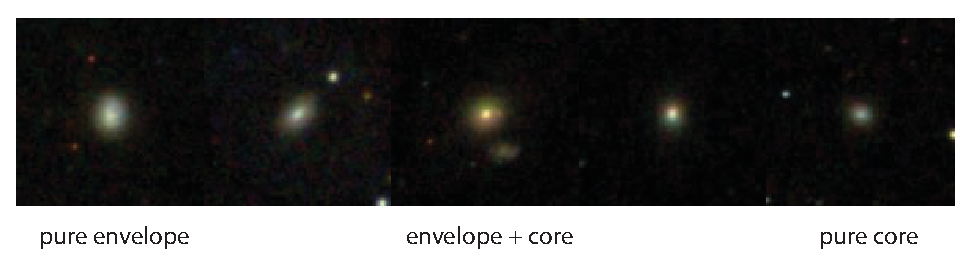
\includegraphics{CCGpics.eps}
\caption{default}
\label{fig:pics}
\end{center}
\end{figure*}

Now that we have seeing-deconvolved \Reff\ values for the entire RESOLVE sample, we begin our search for compact core galaxies. We use the AIMSS sample to select a maximum cutoff core-only radius for CCGs at 800 pc. This upper limit ensures that we are selecting the most compact galaxies in RESOLVE, but also lets us select a range of CSSs, including cEs and dEs. RESOLVE's lower stellar mass limit of  restricts us from reaching down to UCD masses.

We start our search for CCGs by using the one component fit from the above analysis and select galaxies with \Reff\ values $<1000$ pc. Since we are looking for galaxies with compact cores, going up to \Reff\ $\sim 1000$ pc allows us to select objects with cores that are dominating the light and therefore may have a smaller core \Reff\ in a two component fit. We also limit the  $\chi^2/\nu$ to be $<1.3$, since values above this represent galaxies with large residuals left over, which are spirals or irregulars that we would not consider ``cored". After this selection, we are left with 124 galaxies in the CCG candidate sample.

Next, we perform new two component fits using different fitting constraints: (1) the central x and y positions are taken from the one component fit and are held constant for both S\'ersic components, (2) the \Reff\ of the second S\'ersic fit is constrained to always be larger than that of the first S\'ersic fit, and (3) the S\'ersic n of the second component is held constant at 1 for an exponentially decreasing disk profile. We let the values of \Reff, the integrated magnitude, b/a ratio, and PA change for both fits. By doing this, we are forcing \textsc{Galfit} to fit on a core (the first S\'ersic fit) and disky envelope (the second S\'ersic fit) for each CCG candidate.

We then examine the fits by eye and create our final CCG sample by selecting where the core \Reff\ $< 800$ pc and $\chi^2/\nu < 1.3$ to again exclude poor fits. Our sample is thus comprised of 96 CCGs in total (63 from RESOLVE-A and 33 from RESOLVE-B). This represents $\sim6$\% of the total RESOLVE galaxy sample. \autoref{fig:radius} shows their distribution in stellar mass and decomposed \Reff\ compared to other RESOLVE galaxies and the AIMSS cEs and dEs. For the RESOLVE sample, we are plotting the one component fits 

We quantify the amount of light in the core vs. the envelope by taking a ratio of the fluxes of the core and the envelope. The flux of each component is computed with $m = -2.5 \times \log({\rm flux})$, where $m$ is the integrated magnitude output from \textsc{Galfit}. There areWhen \textsc{Galfit} cannot find a core or an envelope, it will sometimes fit instead an extremely large and faint component instead. Where this happens (5 out of 124 cases), we classify this fit as either all core/envelope depending on which component was bad. We also see in 4 out of the 124 cases that the \Reff\ values for each component will be exactly the same value. When this occurs, we classify the galaxy as being all core. 

\begin{figure*}[htbp]
\begin{center}
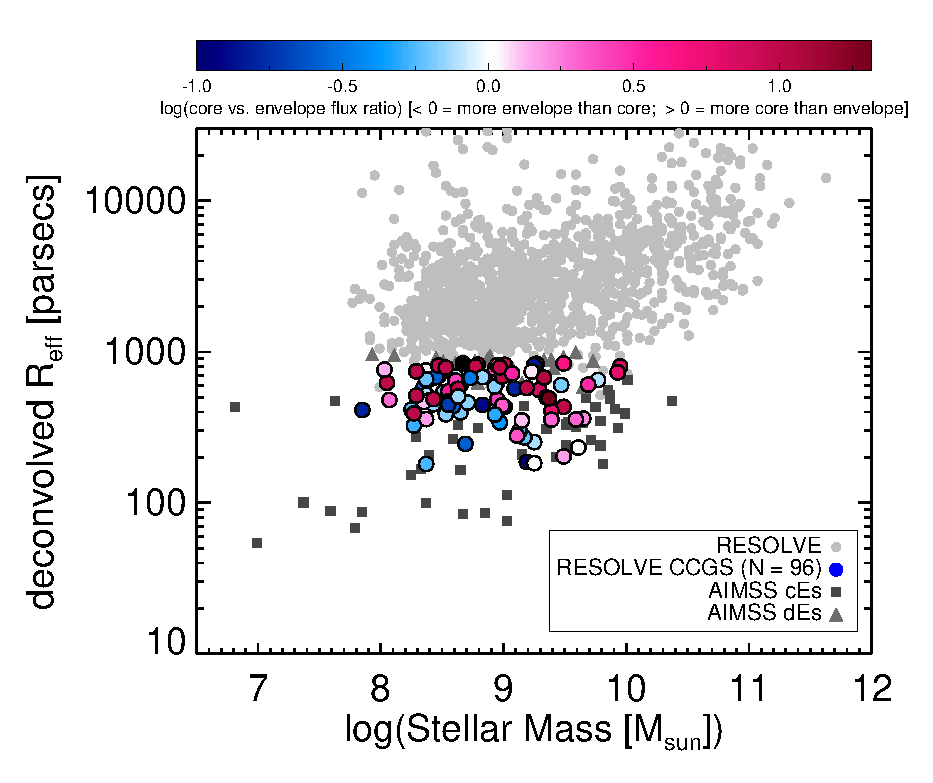
\includegraphics{Reff_Mstars.eps}
\caption{We plot here the deconvolved \Reff\ measurements for the}
\label{fig:radius}
\end{center}
\end{figure*}

\section{Methods}
\label{methods}

\subsection{Photometry: galaxy colors, stellar and baryonic masses, and star formation rates}
\label{phot}
\noindent The RESOLVE survey overlaps with a number of photometric surveys, including GALEX $NUV$ \citep{Morrissey2007}, SDSS-DR8 $ugriz$ \citep{Aihara2011}, and UKIDSS $YHK$ and/or 2MASS $JHK$ \citep{Skrutskie2006}. We reprocess this photometric data in a custom way in order to improve upon the standard SDSS pipeline photometry with improved sky subtraction following Blanton et al. (2011) and use additional sky subtraction for 2MASS and UKIDSS. and use it to derive galaxy colors, stellar and baryonic masses, and star formation rates. \citet{Eckert2015} describes in detail RESOVLE's custom reprocessing for these photometry, but the basic steps are described here. 

Our reprocessed photometry improves over SDSS pipeline photometry in several key ways. First, we use images with improved sky subtraction coming from either Blanton et al. (2011) for SDSS or our own additional sky subtraction for 2MASS and UKIDSS. Second, we use the sum of the high S/N gri images to define the elliptical apertures, allowing us to determine the PA and axial ratio of the outer disk if present. Third, we apply these same elliptical apertures to all bands which allows us to measure magnitudes for galaxies that may not have been detected by the original automated survey pipeline in certain bands, especially low surface brightness galaxies in 2MASS, UKIDSS, and GALEX. Lastly, we use two to three non-parametric methods of total magnitude exrapolation, measuring the light from each band independently (see Figure 2 and 3.1.2). This last point allows for color gradients within galaxies, as opposed to the model magnitudes provided by SDSS (more details in 3.1.3), and allows us to measure systematic errors on magnitudes. We provide a comparison of the magnitudes, colors, and radii with photometry from the DR7 catalog of SDSS in Figure 3 and 3.1.3. Briefly summarizing, we find that the newly reprocessed photometry yields brighter magnitudes and larger effective radii. The colors tend to be bluer for large objects, which we believe to be a consequence of both the improved sky subtraction from Blanton et al. (2011) and the fact that we allow color gradients in magnitude estimation. The newly reprocessed photometry does not create a tight red sequence on the color-magnitude relation as seen in the DR7 photometry, however we argue that the tight red sequence may be a consequence of these two issues in �3.1.3. We also dis- cuss an independent validation of our methods with the NFGS survey (shown in Figure 2a of K13) in 3.1.3.


Stellar masses and star formation rates are then derived from these colors using the stellar population synthesis code described in 

To calculate stellar masses and colors, we use the
spectral energy distribution (SED) modeling code described in Kannappan \& Gawiser (2007), Kannappan et al. (2009), and K13, which fits our newly reprocessed total NUVugrizY JHK magnitudes to a grid of stellar population models. With up to 9 or 10 bands of photo- metric data in ECO and RESOLVE-B respectively, we can estimate robust stellar masses. In RESOLVE-B we exclude the UKIDSS data if they are flagged due to sky background or image artifact issues (E15). We do not use UKIDSS J and we exclude H and K band data if they are fainter than 18 and 17.5 mag respectively. We exclude 2MASS JHK data if they are fainter than 16, 15, and 14.5mag respectively. We exclude any NUV data fainter than 24 mag. In this work we consider two model sets to determine
how robust the mass function shape is to changes in IMF and star formation history. Both model grids consist of an old and young population, yielding a composite stellar population (CSP), including an old population and

\subsection{Environmental Metrics}
\label{env}
\noindent RESOLVE is advantageous to this study because it offers excellent environment information, allowing us to search for CCGs in all environments including groups, clusters, walls, and filaments. We explore the environments of CCGs using two different metrics: the mass of their group halo and their distance to another galaxy. The group halo mass allows us to look for CCGs that are M32--Andromeda analogs where tidal stripping may be at play, or conversely look for CCGs in large groups where ram-pressure stripping could occur. The distance to neighboring galaxies lets us examine if interaction may occur or look for analogs of the isolated galaxies found by \citet{Huxor2013} and \citet{Paudel2014}.

Galaxy groups are identified using the friends-of-friends algorithm of \citet{Berlind2006}, and the masses of these group halos are calculated based on the observed total $r$-band luminosity of galaxies in each group using abundance matching, as described in \citet{Blanton2007}. More information on group identification can be found in \citet{Moffett2015}. The nearest neighbor distances are computed using the RA, Dec, and redshifts of each galaxy and along with spherical geometry principles. 

\subsection{Kinematics}
\label{kin}

\noindent As noted in the Introduction, the velocity dispersion of a galaxy is an extremely helpful tool when testing formation scenarios. We describe the data reduction and analysis to derive $\sigma$ for our CCG sample in this section. 

\subsubsection{SOAR spectroscopy}
\noindent The RESOLVE survey gets the bulk of its spectroscopic data from the SOuthern Astrophysical Research (SOAR) Telescope, located at Cerro Tololo, Chile. We employ the Goodman Spectrograph, designed and built by UNC, along with RESOLVE's custom-built image slicer with 3 $1''$ slits to observe galaxies in both a broad setup and either an emission- or absorption-line kinematic setup. With this absorption-line setup, we are able to derive velocity dispersions. We use the highly-efficient 2100 l/mm VPH grating in order to cover a wavelength range 4858-5503\AA, which includes stellar absorption lines such as H$\beta$, the magnesium triplet, and Fe5270/5335. To achieve S/N $\sim$ 25 per \AA, we bin each central spectrum to \Reff.

The reduction process is as follows: we use standard IRAF tasks to perform bias and overscan subtraction, trimming of the science data to remove unnecessary spatial coverage, and flat fielding. We then use \texttt{LA\_COSMIC} \citep{vanDokkum2001} to clean cosmic rays from each science exposure. We next complete a wavelength calibration and transformation, and then perform object tracing and extraction into a 1D spectrum using the IRAF task apall. We lastly combine the individual exposures using the IRAF task scombine.

\subsubsection{Gemini-South spectroscopy}

\noindent A subset of the smallest galaxies in RESOLVE are observed with the Gemini-South IFU for their kinematics instead of SOAR. For this absorption-line setup, we use the B1200 grating in 1-slit mode to cover a spatial region of 3"$\times$5" and the spectral range 4200-5600\AA. The B1200 grating offers 0.9\AA\ resolution when binned spectrally by 2. We calculate our exposure times such that we achieve S/N $\sim$ 25 per \AA\, after binning by 2 in the spectral direction and summing the fibers out to \Reff.

The spectral reduction proceeds as follows. Using the standard IRAF Gemini-GMOS data packages, bias and overscan subtraction, spatial trimming, flat fielding and fiber identification are performed. We next use the GMOS package gemCRspec, a wrapper for \texttt{LA\_COSMIC}, to clean cosmic rays from each science exposure. We then correct the science frames for quantum efficiency differences between CCDs. Wavelength transformation, sky subtraction, and flux calibration are subsequently performed, and lastly, data cubes are made and summed. We then stack the individual fiber spectra out to \Reff\ to create a 1D spectrum for each galaxy that has S/N $\sim25$. More information on the data reduction for the Gemini GMOS IFU can be found in  Appendix A.

\subsubsection{Velocity Dispersion Extraction}

\noindent We then derive $\sigma$ from the both the SOAR and Gemini spectra using {\sc pPXF}, the penalized pixel fitting code from \citet{Cappellari2004}. This code fits a combination of high-resolution (FWHM $= 0.55$ \AA) ELODIE-based model spectra from \citet{Maraston2011} to the observed input spectrum, and determines a best fit solution for $\sigma$. A caveat to these fits is that they are not corrected for any stellar rotation, which will make absorption lines wider and thus skews the derived $\sigma$ values toward higher values depending on the amount of rotation in each galaxy. Future work will include implementing a stellar rotation subtraction routine for these fits, but preliminary testing by binning the spectra to $1''$ instead of to \Reff\ shows little change between the derived $\sigma$ values.

\begin{figure}[t]
\begin{center}
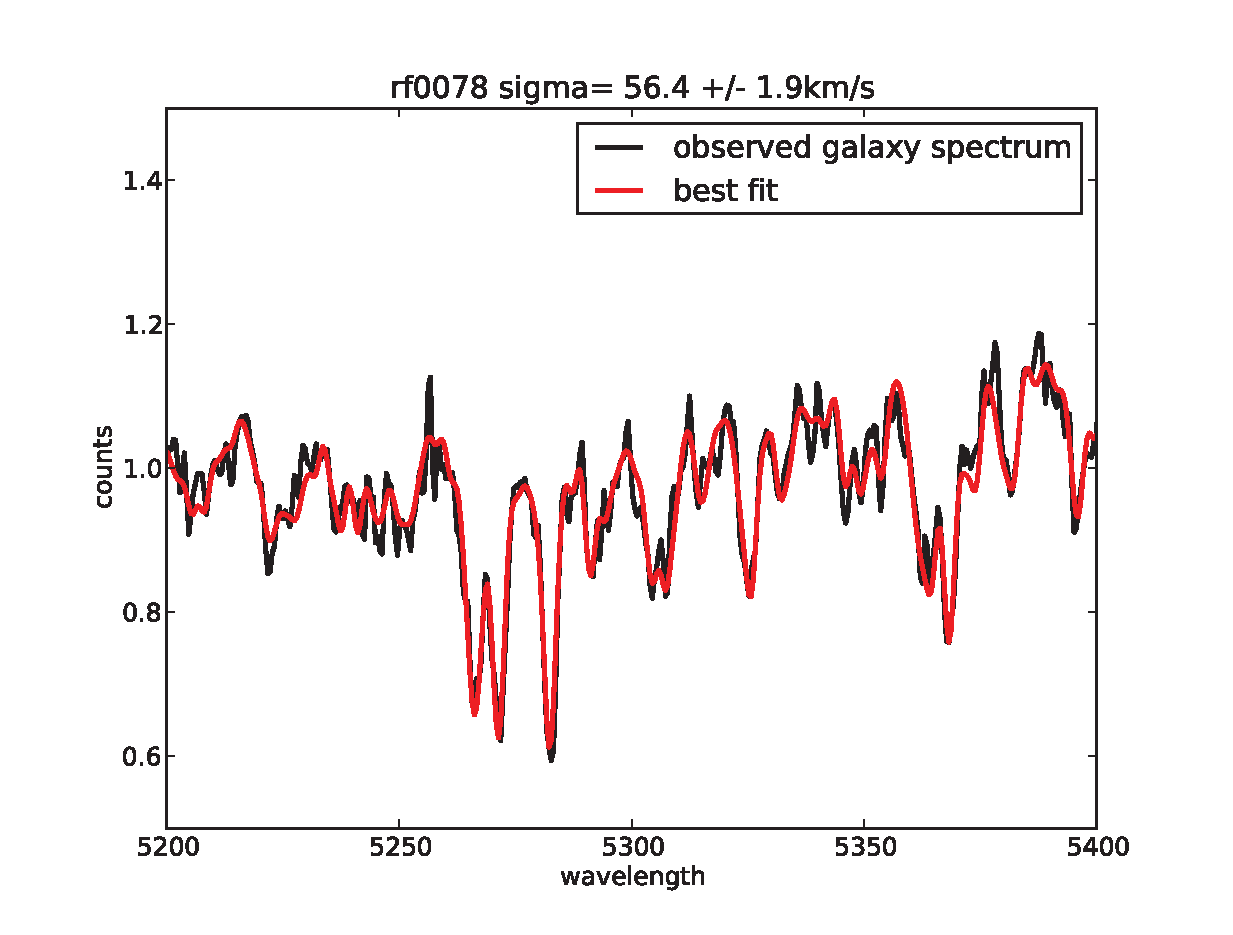
\includegraphics[scale=0.4]{rf0078ppxffit.eps}
\caption{default}
\label{fig:envplot}
\end{center}
\end{figure}

%%%%%%%%%%%%%%%%%%%%%%%%%%%%%%%
%%%%%%%%%%%%%%%%%%%%%%%%%%%%%%%
\section{Results}

\subsection{Colors and Star formation rates}

\begin{figure*}[t!]
\begin{center}
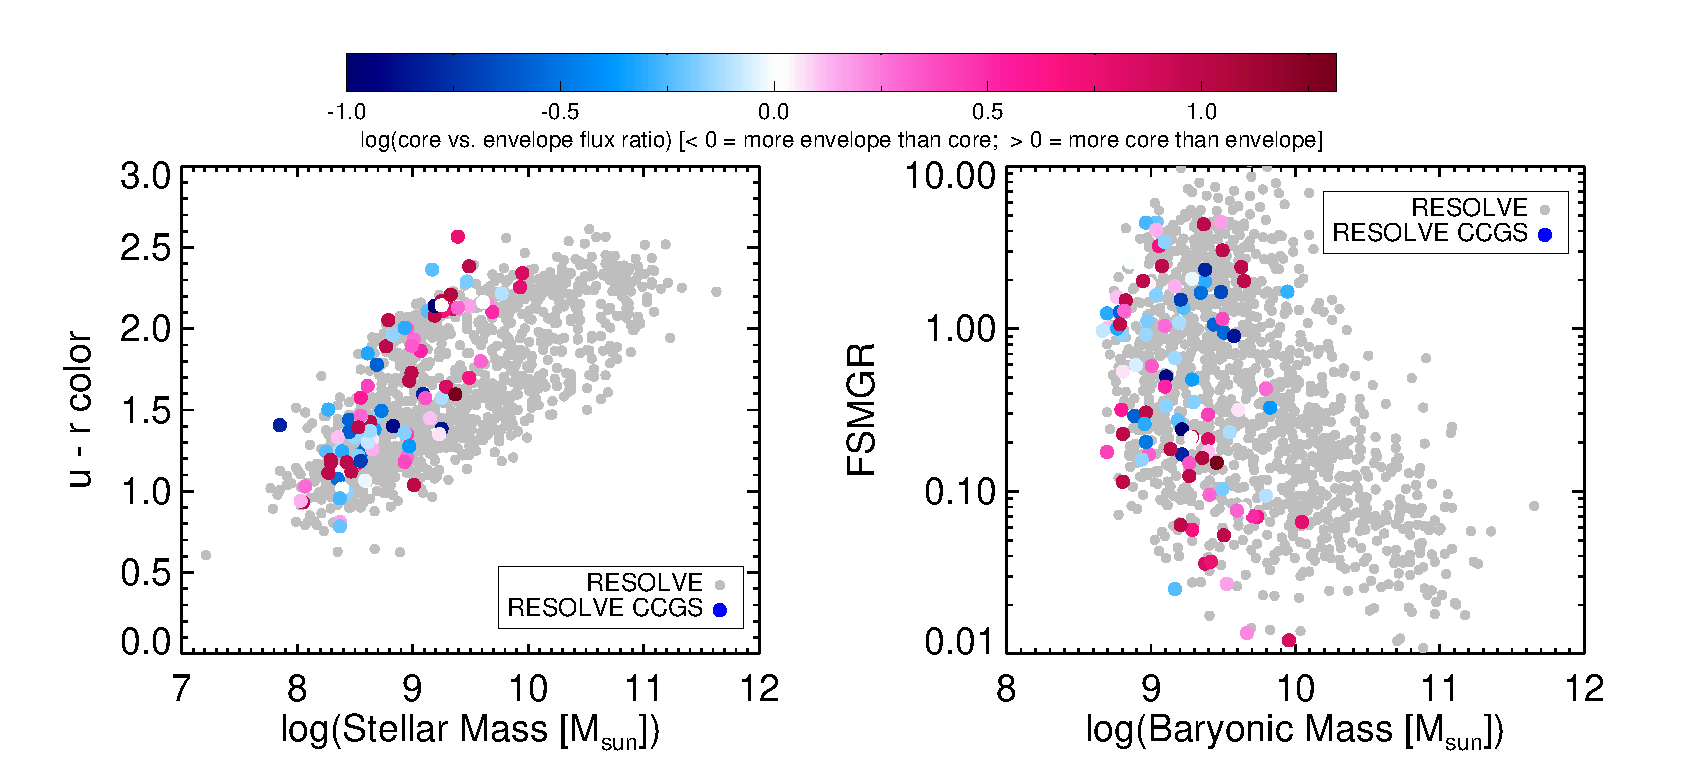
\includegraphics[scale=0.65]{sfr_mbary.eps}
\caption{default}
\label{flg:fsmgr}
\end{center}
\end{figure*}

\noindent The left side of \autoref{fig:envplot} shows the $u-r$ colors of our CCG sample plotted against M$_*$, compared to the RESOLVE sample as a whole. An unusual finding is that many CCGs live on the blue sequence, a previously rare color for CSSs. REF and REF have previously found UCDs in the blue cloud but most cEs and dEs are typically thought of as being "red and dead".

The right side of \autoref{fig:envplot} shows FSMGR vs. M$_{\rm bary}$ for the same objects. As with the colors, we find that many CCGs are forming stars at a rapid rate (> 1 per Gyr). This again goes against the common thought that CSSs are ``red and dead".


\subsection{Environments}
\noindent 
 *FIGURE: nearest neighbor and group halo mass\\
* FIGURE: group n vs group halo mass  \\
* Tie in Huxor's cE, idea of ejection from groups, how environment would effect CCGs

\begin{figure*}[t]
\begin{center}
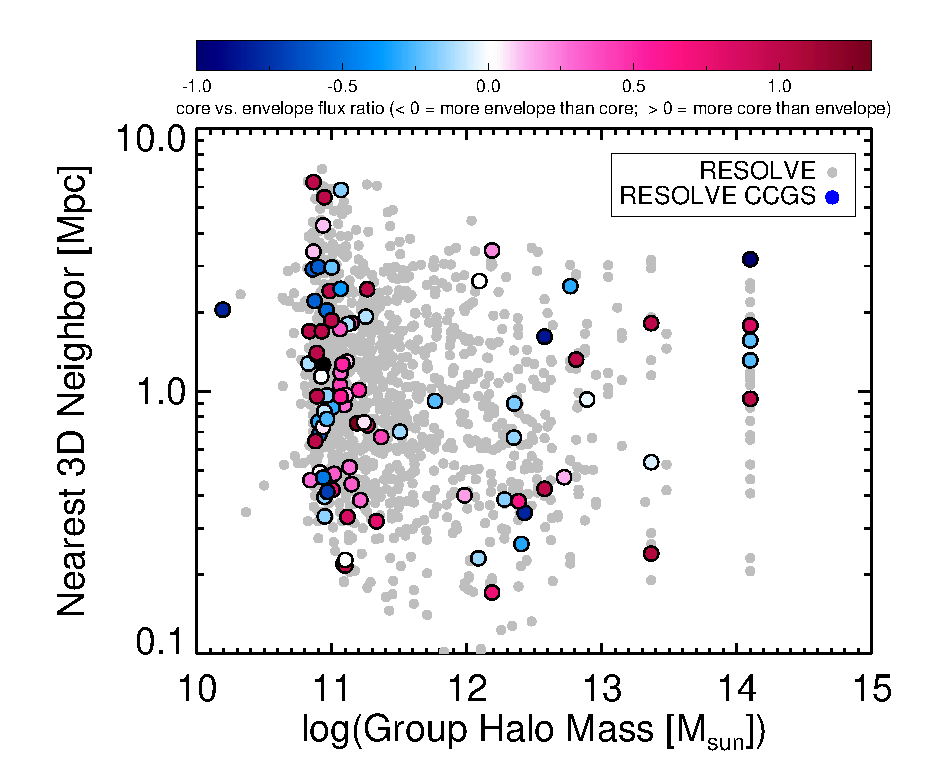
\includegraphics{nn_groupmass.eps}
\caption{default}
\label{fig:envplot}
\end{center}
\end{figure*}

\subsection{Kinematics}
\noindent * why kinematics are important for formation scenario discernment\\
* FIGURE: ppxf fits for spectroscopic data to derive velocity dispersions \\
* FIGURE: velocity dispersion vs. stellar mass

\begin{figure*}[t!]
\begin{center}
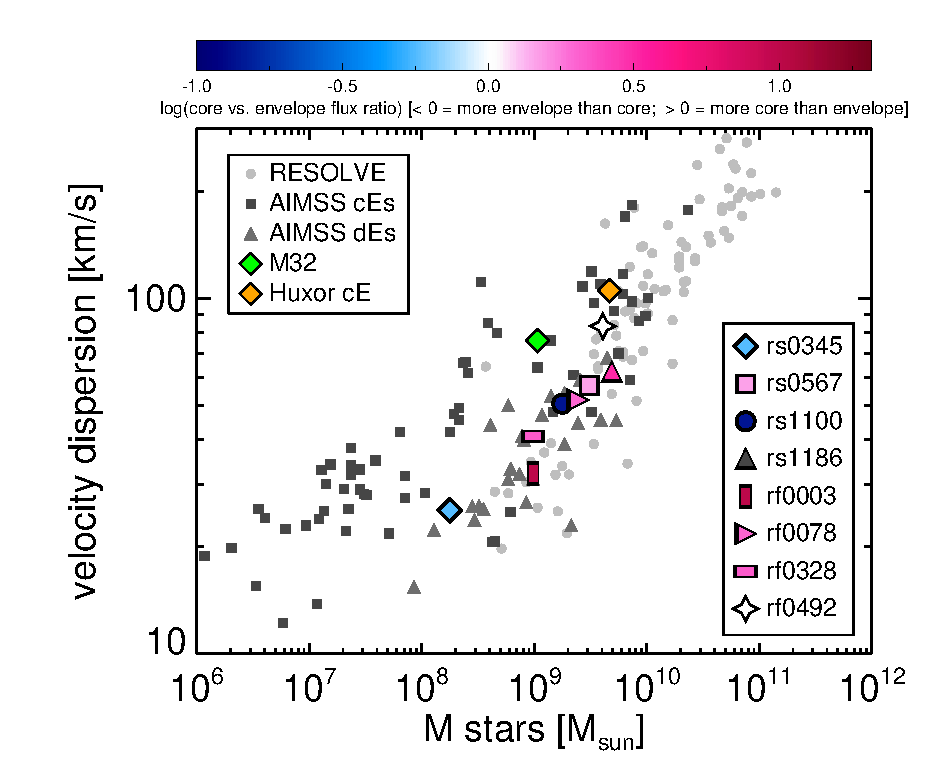
\includegraphics{faber-jackson_resolvesigmas.eps}
\caption{default}
\label{flg:fsmgr}
\end{center}
\end{figure*}

%%%%%%%%%%%%%%%%%%%%%%%%%%%%%%%
%%%%%%%%%%%%%%%%%%%%%%%%%%%%%%%
%\section{CCG formation and evolution} %kind of like a discussion section



%%%%%%%%%%%%%%%%%%%%%%%%%%%%%%%
%%%%%%%%%%%%%%%%%%%%%%%%%%%%%%%
\section{Summary}


\section{Future Work}
%\subsection{Gas Content}
%\noindent * look into g/s ratios \\
%* reference Dave and Katie's work here

%\subsection{Metallicities}
%\noindent * reference AIMSS III paper on what metallicities could tell us about formation scenarios
%%%%%%%%%%%%%%%%%%%%%%%%%%%%%%%
%%%%%%%%%%%%%%%%%%%%%%%%%%%%%%%
\acknowledgments{
  Acknowledgments. 
}

\begin{table*}[b]
\caption{default}
\begin{center}
\begin{tabular}{cccccccc}\hline \hline
\# & name & RA & Dec & core \Reff\ [pc] & envelope \Reff\ [pc] & $\chi^2/\nu$ & log(flux$_{core}$/flux$_{envelope}$) \\ \hline
1 & rs0003 & 133.68635 & 4.3019552 & 821.463 & 821.463 & 1.18600 & 1.00000  \\
2 & rs0178 & 149.91796 & 3.2930701 & 397.295 & 1406.25 & 1.16500 & -0.184240  \\
3 & rs0226 & 153.10508 & 1.2459080 & 632.824 & 3156.16 & 1.21900 & 0.297680  \\
4 & rs0241 & 155.57380 & 0.010365953 & 445.272 & 884.769 & 1.07200 & -0.904000 \\
5 & rs0246 & 155.77914 & 1.0061422 & 533.968 & 1056.30 & 1.08500 & 0.697800 \\
6 & rs0264 & 156.83775 & 0.42236355 & 489.703 & 1015.89 & 1.17800 & -0.292520 \\
7 & rs0284 & 158.11599 & 3.9140821 & 438.697 & 1239.27 & 1.16200 & -0.539200 \\
8 & rs0297 & 159.47069 & 4.8132268 & 712.400 & 768.898 & 1.07100 & -0.568280 \\
9 & rs0345 & 163.22317 & 4.5062644 & 414.999 & 966.451 & 1.06700 & -0.243041 \\
10 & rs0350 & 163.69943 & 2.9479643 & 772.270 & 1584.13 & 0.952000 & 0.394559 \\
11 & rs0364 & 165.21139 & 4.3915459 & 538.817 & 1612.12 & 1.16000 & -0.158081 \\
12 & rs0419 & 169.33097 & 2.8817070 & 252.336 & 1002.62 & 1.03500 & -0.111560 \\
13 & rs0422 & 169.39304 & 2.7726236 & 752.425 & 1189.52 & 1.09100 & 0.0501595 \\
14 & rs0424 & 169.54402 & 2.6007993 & 463.767 & 1092.22 & 1.18400 & -0.672560 \\
15 & rs0485 & 172.24999 & 3.8540120 & 584.173 & 803.029 & 1.17200 & -0.519680 \\
16 & rs0493 & 172.55178 & 3.8010930 & 837.815 & 849.963 & 1.04200 & -0.351080 \\
17 & rs0511 & 173.51621 & 2.9734660 & 650.023 & 1211.75 & 1.04000 & -0.101080 \\
18 & rs0529 & 174.73052 & 3.6007886 & 444.960 & 1989.59 & 1.18600 & -0.142760 \\
19 & rs0541 & 175.29068 & 4.6257403 & 560.561 & 1411.80 & 1.06800 & 0.846080 \\
20 & rs0559 & 176.80368 & 2.5339341 & 460.211 & 1210.71 & 1.11800 & -0.160679 \\
21 & rs0567 & 177.62803 & 1.9833304 & 203.049 & 2150.17 & 1.08800 & 0.165200 \\
22 & rs0586 & 179.25994 & 0.49846395 & 519.351 & 807.097 & 1.12600 & -0.110800 \\
23 & rs0596 & 180.30504 & 2.0499671 & 499.161 & 2119.90 & 1.08000 & 0.856960 \\
24 & rs0623 & 180.73707 & 1.3937952 & 475.008 & 1019.83 & 1.13200 & -0.307200 \\
25 & rs0640 & 180.90099 & 3.7565363 & 571.896 & 1138.14 & 1.14900 & -0.797760 \\
26 & rs0662 & 181.05450 & 1.9002092 & 800.801 & 1212.27 & 1.07800 & 0.867321 \\
27 & rs0663 & 181.06209 & 1.8667357 & 833.690 & 1576.26 & 1.09800 & 0.690200 \\
28 & rs0666 & 181.07212 & 1.9175187 & 432.492 & 432.492 & 0.998000 & 1.00000 \\
29 & rs0685 & 181.15300 & 1.8926987 & 270.945 & 471.503 & 1.02400 & -0.231679 \\
30 & rs0692 & 181.19149 & 1.8039932 & 299.521 & 1419.81 & 1.14800 & -0.238760 \\
31 & rs0693 & 181.19332 & 2.0052805 & 577.377 & 3597.03 & 1.10500 & 1.00000 \\
32 & rs0706 & 181.32842 & 1.6376421 & 186.636 & 854.695 & 1.06100 & -1.00000 \\
33 & rs0744 & 182.42105 & 0.65773495 & 361.692 & 915.910 & 1.00200 & 0.225360 \\
34 & rs0749 & 182.62971 & 0.67284561 & 404.559 & 501.619 & 0.703000 & 0.753240 \\
35 & rs0782 & 183.89462 & 1.2864481 & 450.290 & 848.580 & 1.11100 & -0.164360 \\
36 & rs0812 & 185.76816 & 3.6659076 & 492.992 & 2409.71 & 1.12600 & 1.31604  \\
37 & rs0814 & 185.81878 & 4.8360734 & 480.111 & 1499.67 & 1.15000 & 0.287200 \\
38 & rs0840 & 187.42097 & 0.25347730 & 641.957 & 919.368 & 1.09300 & 0.0679602 \\
39 & rs0862 & 187.93979 & 0.45263727 & 814.029 & 1199.91 & 1.17600 & 0.334680 \\
40 & rs0869 & 188.68743 & 0.36667434 & 352.165 & 1889.67 & 1.21200 & 0.109560 \\
41 & rs0906 & 191.31812 & 2.4491060 & 483.224 & 2456.56 & 1.11800 & 0.419680 \\
42 & rs0972 & 197.87107 & 3.6874893 & 730.731 & 889.397 & 1.00900 & 0.793440 \\
43 & rs0995 & 198.99419 & 2.9514062 & 836.917 & 2778.09 & 1.17400 & 0.653160 \\
44 & rs1001 & 199.42659 & 3.6036901 & 692.197 & 855.021 & 1.13400 & 0.111879 \\
45 & rs1053 & 201.81573 & 4.2087658 & 653.203 & 1401.12 & 1.10500 & 0.00380042 \\
46 & rs1091 & 203.50670 & 1.0961109 & 278.757 & 833.818 & 1.08000 & 0.361680 \\
47 & rs1094 & 203.52381 & 4.7805252 & 796.666 & 5662.08 & 1.09100 & 1.00000 \\
48 & rs1100 & 203.64064 & 4.9188438 & 817.006 & 914.505 & 1.05000 & -0.856239 \\
49 & rs1103 & 203.71245 & 4.2369242 & 358.480 & 1186.76 & 1.14700 & 0.175280 \\
50 & rs1128 & 204.34076 & 4.6890855 & 604.906 & 1514.74 & 1.17300 & 0.135961 \\
51 & rs1359 & 204.71440 & 4.4317127 & 513.871 & 1451.63 & 1.14900 & -0.0193595 \\
52 & rs1172 & 205.14099 & 4.8202809 & 385.743 & 927.874 & 1.12800 & -0.170840 \\
53 & rs1180 & 205.38541 & 4.1942047 & 603.266 & 1102.00 & 1.29500 & -0.188240 \\
54 & rs1186 & 205.49539 & 4.7635971 & 605.924 & 1193.42 & 0.968000 & 0.512960 \\
55 & rs1207 & 206.55280 & 3.5059126 & 432.668 & 1470.88 & 1.05300 & 0.281721 \\
56 & rs1208 & 206.60028 & 1.5787812 & 679.536 & 1019.00 & 1.24500 & -0.584320 \\
57 & rs1257 & 211.35992 & 3.0333434 & 657.017 & 928.701 & 1.09100 & -0.214119 \\
58 & rs1259 & 212.19482 & 4.9098567 & 340.962 & 982.659 & 1.12200 & -0.370719 \\
59 & rs1270 & 216.07293 & 4.6996761 & 587.943 & 1259.93 & 1.08200 & -0.164520 \\
60 & rs1291 & 224.22974 & 4.2051356 & 739.350 & 1137.16 & 1.22400 & 0.0689202 \\
61 & rs0287 & 158.77285 & 0.28142271 & 411.813 & 840.318 & 1.08800 & -0.803640 \\
62 & rs1453 & 200.69881 & 3.7793812 & 324.608 & 792.803 & 1.20200 & -0.284640 \\
63 & rs1456 & 205.20741 & 2.8178559 & 391.510 & 391.510 & 1.08600 & 1.00000 \\
64 & rf0518 & 2.2105393 & -1.1702019 & 465.731 & 2196.11 & 1.13900 & 0.114200 \\
65 & rf0003 & 2.3154592 & 0.81264576 & 686.760 & 686.760 & 0.971000 & 1.00000 \\
66 & rf0078 & 15.724560 & -0.31966061 & 355.476 & 1137.93 & 0.821000 & 0.300120 \\
67 & rf0563 & 16.109272 & -0.65961046 & 822.314 & 3972.25 & 1.17600 & 1.00000 \\
68 & rf0568 & 16.747559 & -0.59600971 & 552.735 & 1257.87 & 1.21100 & -0.313640 \\
69 & rf0143 & 18.353539 & 0.22052619 & 689.135 & 1033.19 & 1.08300 & -0.0775604 \\
70 & rf0154 & 18.903888 & -0.95294103 & 789.710 & 20578.8 & 1.12200 & 1.00000 \\
71 & rf0179 & 21.123601 & -0.36943684 & 549.049 & 2260.41 & 1.26300 & 0.585001 \\
72 & rf0195 & 21.478055 & -0.98781101 & 718.558 & 2522.79 & 1.16500 & 0.523720 \\
73 & rf0197 & 21.556976 & 0.35858673 & 245.635 & 686.455 & 1.08200 & -0.577440 \\
74 & rf0217 & 21.968796 & -0.50420076 & 801.105 & 27583.3 & 1.19900 & 1.00000 \\
75 & rf0229 & 22.801921 & -0.61075471 & 644.919 & 3473.07 & 1.10000 & 0.413480 \\
76 & rf0241 & 23.436054 & 0.95319263 & 623.932 & 945.284 & 1.20000 & 1.00000 \\
77 & rf0243 & 23.531574 & -1.0483175 & 681.056 & 1421.28 & 1.18200 & -0.148561 \\
78 & rf0247 & 23.786680 & 0.71782400 & 569.185 & 1700.14 & 1.14600 & 1.00000 \\
79 & rf0250 & 24.296472 & 0.88248657 & 486.472 & 10812.0 & 1.08600 & 1.00000 \\
80 & rf0253 & 24.678808 & -0.34802671 & 183.131 & 739.562 & 1.15800 & 0.0172801 \\
81 & rf0266 & 28.224302 & -0.90206277 & 181.014 & 693.328 & 1.18200 & -0.262840 \\
82 & rf0280 & 28.693912 & -0.73893120 & 513.218 & 27731.2 & 1.20300 & 1.00000 \\
83 & rf0663 & 34.464996 & 1.2245195 & 762.472 & 2440.96 & 1.19500 & 0.141921 \\
84 & rf0328 & 37.152547 & -0.24656214 & 442.135 & 1714.92 & 1.18400 & 0.339000 \\
85 & rf0332 & 37.413698 & 0.12338943 & 671.104 & 682.327 & 1.27800 & -0.486200 \\
86 & rf0340 & 37.926994 & 1.1969289 & 810.561 & 810.561 & 1.10000 & 1.00000 \\
87 & rf0352 & 38.090155 & 1.1750138 & 675.498 & 1220.81 & 1.13000 & 1.06556 \\
88 & rf0365 & 38.209305 & 0.66106589 & 384.276 & 682.691 & 1.12700 & -0.306679 \\
89 & rf0367 & 38.211703 & 1.1492129 & 471.387 & 1604.43 & 1.16400 & -0.0500407 \\
90 & rf0707 & 40.340884 & 0.058162170 & 464.822 & 1112.55 & 1.14000 & 0.304760 \\
91 & rf0392 & 41.594894 & -1.1714824 & 742.347 & 47400.9 & 1.21200 & 1.00000  \\
92 & rf0419 & 330.45871 & -0.70729601 & 447.720 & 1181.10 & 1.20200 & -0.706640 \\
93 & rf0479 & 353.17151 & -0.75714491 & 507.162 & 1799.10 & 1.18800 & -0.132120 \\
94 & rf0492 & 356.07298 & 0.44182044 & 232.505 & 1118.50 & 1.09600 & 0.00903985 \\
95 & rf0503 & 358.09449 & -0.62866731 & 356.736 & 2299.10 & 0.883000 & 0.314640 \\
96 & rf0505 & 358.63499 & -0.046906637 & 785.406 & 785.406 & 1.17100 & 1.00000 \\

\\ \hline\hline

\end{tabular}
\end{center}
\label{default}
\end{table*}%

\section{Appendix}

\bibliographystyle{apj}
\bibliography{library.bib}


\end{document}
              
